\documentclass[letterpaper]{article}

%%%% ========== PAQUETES NECESARIOS ========== %%%%
\usepackage[utf8]{inputenc} % Codificación de caracteres
\usepackage[spanish]{babel} % Idioma del documento
\usepackage[dvipsnames]{xcolor} % Colores extendidos
\usepackage{amsmath, amssymb, physics} % Matemáticas avanzadas
\usepackage{graphicx} % Insertar imágenes
\usepackage{multicol} % Múltiples columnas
\usepackage{tikz} % Dibujos vectoriales
\usepackage{fancyhdr} % Encabezados y pies de página
\usepackage[colorlinks=true, linkcolor=black,citecolor=black, urlcolor=black]{hyperref} % Hipervínculos
\usepackage[numbers, square]{natbib} % Citas y bibliografía
%%%% ========== CONFIGURACIÓN DE MÁRGENES ========== %%%%
\usepackage{geometry}
\geometry{bottom=2.54cm, top=2.54cm, left=2.54cm, right=2.54cm}

\usepackage{float}
%%%% ========== ENCABEZADOS Y PIES DE PÁGINA ========== %%%%
\pagestyle{fancy}
\fancyhf{}
\fancyhead[R]{Mecánica Clásica}
\fancyhead[L]{\thepage}
\renewcommand{\headrulewidth}{0.08pt}
\renewcommand{\footrulewidth}{0.08pt}
\fancyfoot[L]{}
\fancyfoot[R]{\rightmark}

%%%% ========== COMANDOS PERSONALIZADOS ========== %%%%
\newcommand{\Title}[1]{\begin{center}\LARGE\textbf{\textit{#1}}\end{center}}
\newcommand{\Abstract}[1]{\begin{abstract}\normalsize{#1}\end{abstract}}
\newcommand{\Theorem}[1]{\begin{center}\normalsize\textit{#1}\end{center}}

% Colores personalizados
\newcommand{\blue}{\color{blue}}
\newcommand{\red}{\color{red}}
\newcommand{\green}{\color{OliveGreen}}
\newcommand{\orange}{\color{orange}}

% Atajos matemáticos
\newcommand{\Identity}{\mathbb{I}}
\newcommand{\Reals}{\mathbb{R}}
\newcommand{\Naturals}{\mathbb{N}}
\newcommand{\Integers}{\mathbb{Z}}
\newcommand{\Complex}{\mathbb{C}}

% Operadores matemáticos
\newcommand{\Grad}{\vec{\nabla}}
\newcommand{\Divg}{\vec{\nabla} \cdot}
\newcommand{\Curl}{\vec{\nabla} \times}
\newcommand{\Lapl}{\nabla^{2}}

% Derivadas y operadores
\newcommand{\Partial}[2]{\frac{\partial#1}{\partial#2}}
\newcommand{\SecPartial}[3]{\frac{\partial^{2}#1}{\partial#2\partial#3}}

% Ecuaciones de movimiento
\newcommand{\eqLagrange}[1]{\frac{d}{dt}\cbk{\Partial[\dot{#1}]{\Lag}} - \Partial[#1]{\Lag} = 0}
\newcommand{\Ham}{\mathcal{H}}
\newcommand{\eqHamilton}[2]{\Partial[#1_{i}]{\Ham} = - \dot{#2}_{i}, \quad \Partial[#2_{i}]{\Ham} = \dot{#1}_{i}}

\setlength{\parindent}{0pt}
\setlength{\parskip}{1em} 

\begin{document}

\Title{Evoluci\'on de un rasgo cuantitativo en una poblaci\'on monom\'orfica, enfoque con formalismo de Hamilton-Jacobi.}
\Abstract{El presente trabajo constituye el proyeccto final del curso de \textit{Mecánica Clásica} del primer semestre del programa de \textit{Maestría en Física} del \textit{Instituto de Física de la Universidad Autónoma de Puebla}. En el mismo se trata el tema de \textit{dinámica adaptativa}.}

\begingroup
\setlength{\parindent}{1.5em}
\setlength{\parskip}{0pt}
\tableofcontents
\endgroup
\clearpage

\section{¿Qué es la Dinámica Adaptativa?}

\subsection{Adaptación y Evolución de los Sistemas Biológicos.}

En el estudio de los sistemas biológicos, los conceptos de adaptación y evolución son fundamentales para comprender cómo los organismos responden a su entorno y cómo estas respuestas moldean la diversidad de la vida en la Tierra. \citep{adaptacion} La adaptación se refiere al proceso mediante el cual los organismos desarrollan características que mejoran su capacidad para sobrevivir y reproducirse en condiciones ambientales específicas. Estas características pueden ser de naturaleza física, como la presencia de pelaje grueso en animales que habitan regiones frías; fisiológica, como la capacidad de las plantas desérticas para retener agua; o conductual, como la migración estacional de las aves. La adaptación resulta principalmente de la selección natural, un mecanismo que favorece aquellas variaciones genéticas que proporcionan ventajas competitivas en un entorno particular.

\citep{evolucion} Por otro lado, la evolución es un proceso a largo plazo que describe los cambios genéticos acumulativos en las poblaciones de organismos a lo largo de generaciones. Este fenómeno, impulsado por la selección natural, las mutaciones genéticas, la deriva genética y el flujo génico, es responsable de la aparición de nuevas especies y de la vasta diversidad de formas de vida observada hoy en día. La evolución permite entender cómo los organismos han cambiado con el tiempo para adaptarse a condiciones ambientales cambiantes, y cómo estos cambios han contribuido al desarrollo de estructuras, comportamientos y funciones altamente especializadas.

La relación entre adaptación y evolución es íntima y complementaria. Mientras que la adaptación representa la respuesta inmediata de un organismo o una población a presiones selectivas específicas, la evolución engloba los cambios genéticos a largo plazo que consolidan estas adaptaciones en las poblaciones. Por ejemplo, el cuello largo de las jirafas modernas es el resultado de un proceso evolutivo que tuvo su origen en la ventaja adaptativa de alcanzar las hojas altas de los árboles en entornos de escasez alimentaria.

En el contexto evolutivo, es importante entender los conceptos de genotipo y fenotipo, pues la interacción entre ellos permite que los organismos se adapten a condiciones cambiantes.

El genotipo de un organismo se refiere al conjunto específico de genes que posee, determinado por los cromosomas que hereda. Es la base genética que define las características potenciales de un organismo. En especies asexuales y sexuales haploides, el genotipo se representa por un cromosoma de cada tipo, mientras que en especies diploides esta formado por pares de cromosomas homólogos.

Cualquier característica de un individuo que est e determinada (en alguna medida) por el genotipo se denomina fenotipo (o rasgo fenotípico) y, por ende, es una característica heredable de los padres a la descendencia.

Casi cualquier tipo de característica imaginable depende de los genes, desde rasgos físicos, como el tamaño del cuerpo o los colores, hasta rasgos mentales, como el carácter, la disposición y la inteligencia. Los fenotipos pueden ser discretos, cuando presentan diferencias claras y definidas (por ejemplo el tipo de sangre), o continuos, cuando varían en un rango medible (como la altura o peso \citep{Dercole}).

La variabilidad fenotípica dentro de las poblaciones, conocida como polimorfismo, es crucial para la evolución y la adaptación de los organismos. Los fenotipos discretos suelen depender de uno o pocos genes y tienen poca influencia del ambiente, mientras que los fenotipos continuos están influenciados tanto por multiples genes como por el entorno. Los fenotipos que proporcionan ventajas adaptativas son seleccionados de manera natural, lo que, con el tiempo, lleva a cambios genéticos en la población. Así, la variabilidad genética y fenotípica es esencial para la supervivencia y la evolución de las especies frente a desafíos ambientales y presiones selectivas \citep{Dercole}.

\citep{Mirrahimi2011} Desde la década de 1980, el término \textit{evolución adaptativa} se ha acuñado para describir los formalismos matemáticos que abordan la selección y evolución de un rasgo en una población estructurada por un rasgo fenotípico continuo. Dichos modelos se basan en tres principios fundamentales que sustentan la evolución Darwineana:

\begin{itemize}
	\item {

	      {La multiplicación de la población.}

	      }

	\item {

	      {La selección mediante competencia por los recursos disponibles.}
	      }

	\item {

	      {Mutaciones.}

	      }
\end{itemize}

Modelos simples basados en estos principios pueden explicar como emergen rasgos mas aptos y, a su vez, como poblaciones caracterizadas por varios rasgos bien diferenciados pueden coexistir potencialmente. Las simulaciones numéricas pueden presentar la aparición de ciclos y la especiacion, esto debido a que los recursos limitados generan competencia; los individuos con características similares utilizan recursos similares, dando asi, una competencia mayor entre ellos. La cuestión de comprender cómo, en un población de este tipo, una especie mutante puede invadir o no una población inicial. En modelos de población cerrada, las mutaciones forman parte de la dinámica y se toman en cuenta la heredad de los rasgos ligeramente diferente a los progenitores.

\subsection{Motivación para Introducir la Teoría de Hamilton-Jacobi.}

\citep{barles2007} Las ecuaciones de Hamilton-Jacobi son herramientas útiles para describir diversas asintóticas singulares, es decir, situaciones en las que el comportamiento de un sistema físico o matemático cambia  de manera abrupta o presenta características extremas en ciertas condiciones, como cerca de puntos críticos, bordes o zonas donde se manifiestan discontinuidades. Estas presentan soluciones límite o aproximadas en condiciones extremas.


En los sistemas ecológicos y biológicos, la adaptación y evolución son procesos fundamentales que determinan la dinámica y supervivencia de las poblaciones. La capacidad de las especies para adaptarse a cambios en su entorno a través de la selección natural, la mutación y la competencia es un tema central en biología teórica. Para modelar estos procesos, las ecuaciones de Hamilton-Jacobi (H-J) han emergido como herramientas matemáticas poderosas para describir la evolución de poblaciones bajo distintos escenarios ecológicos.

\citep{Mirrahimi2011}El ejemplo mas simple para un modelo matemático autocontenido para la evolución adaptativa es el quimiostato. Microorganismos caracterizados por un parámetro $x$ viven en un bao que contiene un nutriente continuamente renovado a una tasa $d>0$. Esta concentración se denota por $S(t)\geq0$ (para el sustrato), y el nutriente fresco se denota por $S(t)_{in}\geq0$. La densidad de población del microorganismo es $n(x,t)$, y la tasa de absorción para los individuos con rasgo $x$ es $\eta(x)>0$. Dando así las ecuaciones:

\begin{equation*}
	\left\{\begin{array}{l}
		\frac{d S(t)}{d t}=d\left(S_{i n}-S(t)\right)-S(t) \int_{-\infty}^{\infty} \eta(x) n(x, t) d x, \\
		\frac{\partial n(x, t)}{\partial t}=-d n(x, t)+(1-\mu) S(t) \eta(x) n(x, t)+\mu S(t) \int_{-\infty}^{\infty} M(y, x) \eta(y) n(y, t) d y
	\end{array}\right.
\end{equation*}

Los dos primeros principios mencionados en la teoría de Darwin están directamente incluidos en el modelo: el crecimiento de la población proviene de la ecuación de $n(x, t)$, y la competencia proviene de la cantidad limitada de nutrientes. Suponemos que inicialmente $S(0) \leq S_{i n}$, por lo que a lo largo de la dinámica $S(t) \leq S_{i n}$, ya que $S(t)$ disminuye si alcanza $S_{i n}$. El término (1$\mu) \eta(x) n(x, t)$ representa la tasa de nacimiento sin mutaciones. El parámetro $0<\mu<1$ representa la proporción de nacimientos que sufren mutaciones.

Las mutaciones están representadas por la probabilidad $M(y, x)$ de que un recién nacido tenga el rasgo $x$ cuando su progenitor tiene el rasgo $y$. Suponemos que $M(y, x) \geq 0$ y $\int_{-\infty}^{\infty} M(y, x) d x=1$

Este modelo se puede simplificar suponiendo que los nutrientes llegan rápidamente a un estado de equilibrio en comparación con la escala temporal de la evolución de la población. Esto se logra reemplazando la ecuación diferencial para $S(t)$ por:

\begin{equation*}
	S(t)=\frac{d S_{\text {in }}}{d+\int_{-\infty}^{\infty} \eta(x) n(x, t) d x} .
\end{equation*}

a su vez, reemplazamos el término de mutación por una ecuación de mutación-difusión:

\begin{equation*}
	\frac{\partial n(x, t)}{\partial t}=-d n(x, t)+S(t) \eta(x) n(x, t)+\lambda \Delta n(x, t) .
\end{equation*}

Con ello podemos construir un sistema de ecuaciones mas generales que pueden considerar tasas de crecimiento con/sin muerte $R(x,I(t)$:

\begin{equation*}
	\left\{\begin{array}{l}
		\frac{\partial n(x, t)}{\partial t}=n(x, t) R(x, I(t))+\lambda \Delta n(x, t), \quad x \in \mathbb{R}, t>0 \\
		I(t)=\int_{-\infty}^{\infty} \eta(x) n(x, t) d x
	\end{array}\right.
\end{equation*}

donde:

\begin{equation*}
	R(x,I)=-d+\frac{dS_{in}}{d+I}\eta(x)
\end{equation*}

\citep{Mirrahimi2011}Tales modelos parabólicos no pueden exhibir altas concentraciones mientras el coeficiente e difusión $\mu>0$ este fijo. Para ello, reescalamos el problema fijando un $\lambda=\varepsilon^2$. Asumiendo que la tasa de mutación es pequeña, considerando el paso al límite $\varepsilon \rightarrow 0$, lo cual lleva a la misma ecuación con $\lambda=0$, el modelo de selección. Esto es debió a que los efectos de mutación requieren tiempo muy prolongados para observarlos, por consiguiente, cambiamos $t$ por $t/\varepsilon$. Por consiguiente, las ecuaciones se transforman:

\begin{equation}
	\left\{\begin{array}{l}
		\frac{\partial n(x, t)_\varepsilon}{\partial t}=n(x, t)_\varepsilon R(x, I_\varepsilon(t))+ \varepsilon^2 \Delta n(x, t), \quad x \in \mathbb{R}, t>0 \\
		I_\varepsilon(t)=\int_{-\infty}^{\infty} \eta(x) n_\varepsilon(x, t) d x .
	\end{array}\right.
\end{equation}

Por otro lado, se puede demostrar bajo las condiciones:

\begin{equation*}
	\begin{cases}
		\sup_{x \in \mathbb{R}} R(x, I_M) = 0, \\
		\min_{x \in \mathbb{R}} R(x, I_m) = 0, \\
		\forall I \geq 0, \, R_I(x, I) < 0.
	\end{cases}
\end{equation*}

\begin{equation*}
	0< \eta_m \leq \eta(x) \leq \eta_M < \infty
\end{equation*}

Se puede demostrar que si $R$ es monótona en $x$ con datos iniciales "bien preparados", existen dos constantes $\rho_m >0$ y $\rho_M >0$, tales que:

\begin{equation*}
	\rho_m \leq \int_{-\infty}^{\infty} n_\varepsilon(x,t) \, dx \leq \rho_M
\end{equation*}

La demostración del Teorema anterior utiliza el método WKB, común en la propagación de frentes, aplicado en dinámica adaptativa. Este enfoque introduce una nueva ecuación de Hamilton-Jacobi debido a una restricción algebraica. La clave es la transformación de Hopf-Cole:

\begin{equation}
	u_\varepsilon = \varepsilon \ln(n_\varepsilon)
\end{equation}


Para esto, los datos iniciales deben estar ``bien preparados'', es decir, concentrados exponencialmente como \( u_0^\varepsilon = \varepsilon \ln(n_0^\varepsilon) \), con \( u_0^\varepsilon \) bien definido cuando \( \varepsilon \to 0 \). Esto lleva a la siguiente ecuación:

\begin{equation*}
	\frac{\partial u_\varepsilon}{\partial t} = R(x, I_\varepsilon(t)) +   \varepsilon \Delta u_\varepsilon + |\nabla u_\varepsilon|^2
\end{equation*}

Se puede demostrar que \( u_\varepsilon \) es uniformemente Lipschitz si \( u_0^\varepsilon \) también lo es, y que \( I_\varepsilon \) tiene variaciones acotadas. Al hacer \( \varepsilon \to 0 \), obtenemos la ecuación de Hamilton-Jacobi restringida:


\begin{equation*}
	\begin{cases}
		\frac{\partial u}{\partial t} = R(x, I(t)) + |\nabla u|^2 \\
		\max_{x \in \mathbb{R}} u(x, t) = 0, \quad \forall t > 0
	\end{cases}
\end{equation*}


La restricción \( \max_{x \in \mathbb{R}} u(x, t) = 0 \) proviene de la cota uniforme sobre la masa total establecida previamente. La solución \( u(x,t) \) se interpreta como solución de viscosidad.

\citep{Mirrahimi2011}En un quimiostato, la competencia entre especies es global y equitativa, pues todos se "alimentan" del único sustrato $S(t)$ introducido. Sin embargo, esto no siempre es el caso, en una situación más realista esta competencia no es equitativa, pues puede ser que un individuo con rasgos más cercanos tengan mayor habilidad de competencia. Para implementar esto, la dinámica población se modela con base a las ecuación tipo Lotka-Volterra:

\begin{equation*}
	\frac{\partial}{\partial t} n(x,t) - \lambda \frac{\partial^2}{\partial x^2} n(x,t) = n(x,t) \left( R(x) - (K * n)(x,t) \right), \quad t \geq 0, \, x \in \mathbb{R}
\end{equation*}

con la condición inicial $n(x,t=0)=n_0(x)$

Cuyos elementos tienen la siguiente interpretación:

\begin{itemize}
	\item \( n(x,t) \): densidad de población en la posición \( x \) y en el tiempo \( t \),
	\item \( R(x) > 0 \): tasa de crecimiento intrínseca de los individuos con el rasgo \( x \) (si están aislados y sin competencia),
	\item \( K \in L^\infty(\mathbb{R}) \): núcleo de competencia, una densidad de probabilidad tal que \( K \geq 0 \) y
	      \[
		      \int_{-\infty}^{\infty} K(z) \, dz = 1,
	      \]
	\item La convolución
	      \[
		      (K * n)(x,t) = \int_{-\infty}^{\infty} K(x - y) n(y,t) \, dy
	      \]
	      representa la competencia por recursos,
	\item \( \lambda \): tasa de mutación, asumida constante.
\end{itemize}
\section{Conceptos Preliminares}
\subsection{Acervo Genético, y Poblaciones Monomórficas y Dimórficas.}

La \textit{reserva genética} o \textit{acervo genético} de una población se define como los alelos\footnote{Un alelo es una de las versiones de una secuencia de ADN que se encuentra en una posición determinada de un cromosoma} de los genes encontrados en los individuos. Cada gen, a su vez, puede contar con su propio acervo genético, el cuál es constituido por lo alelos del mismo. Un ejemplo de esto es una población en la que cada individuo puede ser considerado como un ser único desde el punto de vista genético. Para cada alelo podríamos determinar la frecuencia de aparición, cantidad a la que llamamos frecuencia génica, y esta puede ser expresada como un porcentaje y representa la abundancia del alelo en relación a las otras versiones del su correspondiente gen. Supongamos una población con distintos tipos de alelos del gen $A$, digamos $A$y $A'$, el caso de ser sólo dos. Si esta población cuenta con 100 individuos, estos existen 200 alelos. Suponiendo que aparecen 120 alelos $A$ y 80 alelos $A'$, entonces las frecuencias génicas son 60\% y 40\% respectivamente.

Bajo este entendido, decimos que una población es genéticamente estable, o está en equilibrio genético, cuándo el acervo genético se mantiene constante en el tiempo. Si por el contrario, el acervo cambia de una generación a otra, la población está en \textit{trance evolutivo}. Así pues, las poblaciones genéticamente estables son una hipótesis. Estas fueros descritas por Hardy y Weinberg en 1908, quienes postularon que para que esto se cumpla, deben mantenerse las siguientes condiciones:

\begin{itemize}
	\item

	      La población deber ser muy grande, tal que un cambio fortuito no tenga impacto en su composición genética.



	\item

	      El apareamiento debe ser al azar, esto con motivo de que no haya \textit{favoritismo} hacia ciertas características, que son las que serán heredadas.



	\item

	      No debe haber mutaciones para que el acervo genético no cambie.



	\item

	      No debe haber selección natural, por lo que todos los genotipos\footnote{El genotipo es el conjunto de genes y la información genética que caracteriza a un individuo, y que se transmite de generación en generación} están en igualdad de condiciones con respecto a la reproducción y a la adaptación ambiental.



	\item

	      No debe haber migraciones, es decir, no debe haber flujo genético ni hacia dentro ni hacia afuera de la población.
\end{itemize}

No es difícil deducir qué condiciones deben darse para que la población entre en trance evolutivo.

\begin{itemize}
	\item

	      Poblaciones pequeñas.



	\item

	      Apareamiento selectivo.



	\item

	      Presencia de mutaciones.



	\item

	      Selección natural.



	\item

	      Migraciones, tanto internas como externas.


\end{itemize}

Puestos en este contexto podemos definir a las poblaciones monomórficas y dimórficas.

\textbf{Población Monomórfica:} decimos que una población es monomórfica cuando ésta presenta un sólo alelo para un gen específico. En este contexto decimos que todos los individuos son genéticamente idénticos respecto a dicho gen.

\textbf{Población Dimórfica:} decimos que una población es dimórfica cuando ésta presenta dos variaciones, o alelos en un gen específico.

Estas ideas pueden generalizarse a poblaciones polimórficas, siendo éstas aquellas que presentan un dos o más variaciones, o alelos, de un gen en partícular, pero a efectos de este trabajo, sólo nos resultarán de interés las monomórficas, y las dimórficas.

\subsection{\textit{Chemostat}}

El \textit{chemostat} o \textit{quimiostato} es un dispositivo de laboratorio que está diseñado para el estudio del crecimiento de microorganismos en un ambiente controlado, en un medio líquido. Este dispositivo funciona de la siguiente forma: a un recipiente de vidrio cerrado, de entre 1 mL y unos pocos litros, se le suministra un medio fresco a través de una bomba de afluente. Para mantener un volumen constante, una segunda bomba extrae el líquido a la misma velocidad. Los microorganismos que han sido añadidos al recipiente únicamente pueden alimentarse del la bomba de afluente, y la tasa de crecimiento de esta está definida como la relación entre la tasa de afluente y el volumen del recipiente. Entre los sustratos y factores de crecimiento añadidos al medio, uno es el llamado sustrato de control, que limita el crecimiento.

\begin{center}
	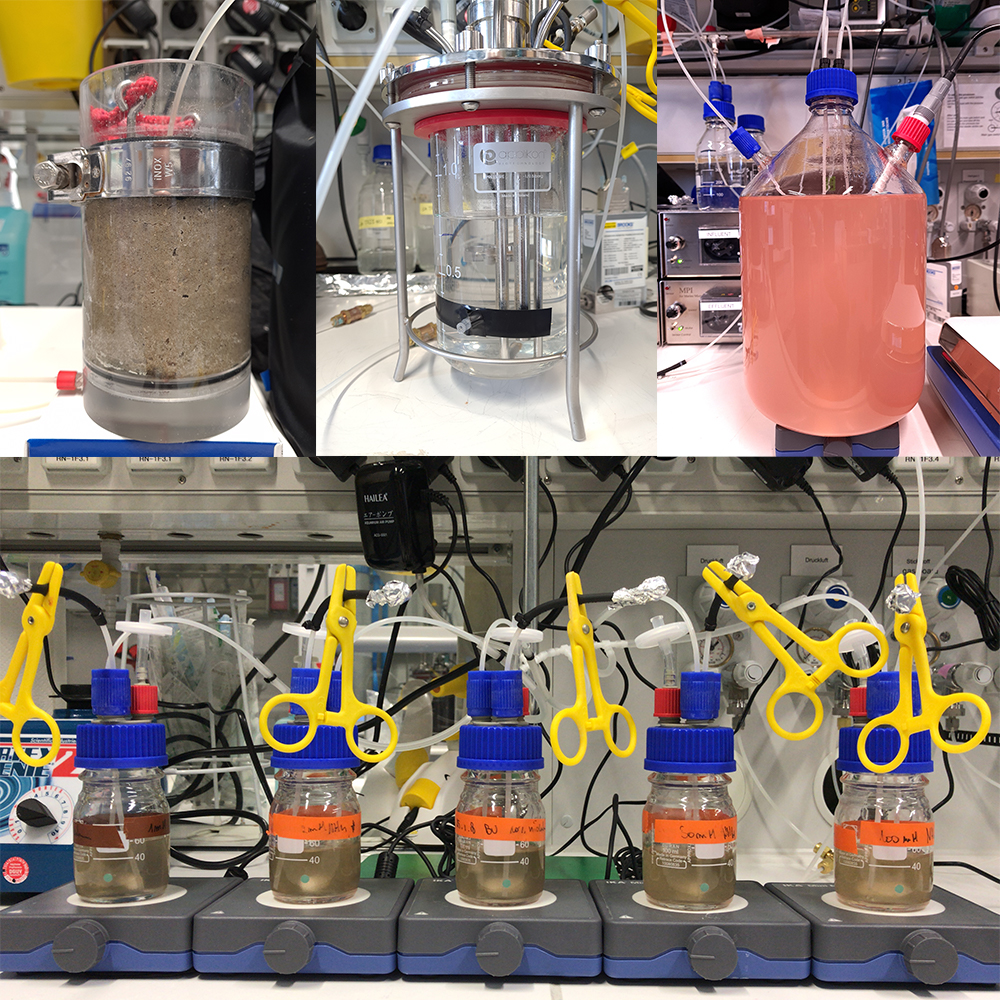
\includegraphics[scale=0.2]{Chemostat.jpg}
\end{center}

Un quimiostato es una buena opción para el cultivo de microorganismos, ya que establecemos condiciones que permanecen constantes, contra los cultivos hechos en lotes. Esto facilita enormemente la reproducción de los experimentos. Algunas de las utilidades del quimiostato son que puede ser utilizado en cultivos puros para el estudio de la cinética del crecimiento microbiano, o para enfoques ómicos más detallados. También se puede utilizar para experimentos de competición.

En estos experimentos se liberan en el recipiente dos o tres microorganismos diferentes, con nichos comparables en condiciones variables; con tasas de crecimiento altas o bajas; con concentraciones de oxígeno altas o bajas; distintos valores de pH o temperatura; con o sin factores de crecimiento, etc.

\subsubsection{GREENT}

La  actividad humana ha tenido serios impactos en los ciclos biológicos del carbono y nitrógeno, y como consecuencia, el calentamiento global y la contaminación del agua. En este contexto, las tecnologías relacionadas con el tratamiento de agua ha mejorado en las últimas décadas. En particular, el uso de anammox (bacterias anaeróbicas oxidantes de amonio) en gránulos con oxígeno tiene el potencial de convertir las tratadoras de agua en sistemas enérgicamente eficientes con mínima emisión de gases de efecto invernadero.

Existen microorganismos que acoplan la oxidación anaeróbica del metano con la desnitrificación. Una integración innovadora de estos en determinados sistemas de tratamiento de aguas podría ofrecer una solución elegante y eficiente para combatir las emisiones de gases de efecto invernadero de las mismas.

El propósito del \textit{GREENT}, o \textit{Mitigación de Gases de Efecto Invernadero Mediante Tecnología Avanzada de Eliminación de Nitrógeno} (por sus siglas en inglés) es determinar las emisiones de óxido nitroso en los bioreactores de nitritación parcial-anammox, y los parámetros que las gobiernan, e investigar las vías responsables con un detalle molecular. Aunado a ésto, también explorar la viabilidad de un bioreactor que elimine el amonio y metano de manera simultanea mediante anammox, y microorganismos anaeróbicos oxidantes de metano.

\subsection{Ecuación de Hamilton-Jacobi, Viscosidad y Constricciones.}
\section{Modelo}
\subsection{Descripción del Entorno Biológico.}

Consideremos un organismo que tiene que proporcionan energía (tales recursos se denominan sustituibles). Sean $S_1$ y $S_2$ las concentraciones de estos dos recursos contenidos en un quimiostato. Entonces el vector:

\begin{equation}
	I=\binom{S_{1}}{S_{2}},
\end{equation}

constituye la condición ambiental [7,8].

Los organismos pueden caracterizarse por diversos grados de consumir. Describimos estos rasgos por x y varían continuamente entre 0 y 1. Si el rasgo toma el valor 0, sólo se consume el recurso $S_2$ y cuando el rasgo toma el valor de 1 solo se consume el recurso $S_1$. El efecto general en el cual contribuyen los dos rasgos se describe a partir de los coeficientes $\eta(x)$  y $\xi(x)$, en el cual la cantidad promedio que consume un organismo con el rasgo x para los recursos 1 y 2 viene dado como:  $\eta(x)$ $S_1$ y $\xi(x)$ $S_2$ respectivamente.

En el caso de una población consumidora monomórfica, la dinámica ecológica está gobernada por el siguiente sistema de ecuaciones diferenciales:

\begin{equation}
	\begin{split}
		\frac{d S_1}{dx} & =S_{01}-S_1-\eta(x)S_1X \\  \frac{d S_2}{dx}&=S_{02}-S_2-\xi(x)S_2X\\ \frac{d S_1}{dx}&=-X+\eta(x)S_1X-\xi(x)S_2X
	\end{split}
\end{equation}

Donde X representa la densidad de la población consumidora y $S_{01}$ es la concentración del recurso i en el medio de entrada.
El sistema ecuaciones (2) tiene siempre que cumplir:

\begin{equation}
	\eta(x)S_1X-\xi(x)S_2X>1,
\end{equation}

y la tasa de crecimiento poblacional de los consumidores con el rasgo X, bajo condiciones ambientales constantes I, está dada por:

\begin{equation}
	r(x,I)=-1+\eta(x)S_1X+\xi(x)S_2X.
\end{equation}

Ahora, el análogo de (2) para la competencia de dos poblaciones consumidoras, una con el rasgo x y la otra con el rasgo y, está dado por el siguiente sistema:

\begin{equation}
	\begin{split}
		\frac{d S_1}{dt} & =S_{01}-S_1-\eta(x)S_1X_1-\eta(y)S_1X_2 \\  \frac{d S_2}{dt}&=S_{02}-S_2-\xi(x)S_2X_1-\xi(y)S_2X_2\\ \frac{d X_1}{dx}&=-X_1+\eta(x)S_1X_1+\xi(x)S_2X_1\\
		\frac{d X_2}{dx} & =-X_2+\eta(y)S_1X_2+\xi(y)S_2X_1
	\end{split}
\label{eq:S-M}
\end{equation}

En el estado estacionario, tanto como r(x,I) y r(y,I) son iguales a cero. Estas son dos ecuaciones lineales con dos incógnitas, $S_1$ y $S_2$. La solución se expresa como:

\begin{equation}
	\binom{S_1}{S_2}=\frac{1}{\eta(x)\xi(y)-\eta(y)\xi(x)}\binom{\xi(y)-\xi(x)}{\eta(y)-\eta(x)}
\end{equation}


A continuación, las dos relaciones de retroalimentación pueden utilizarse para deducir que las densidades en estado estacionario de las dos poblaciones consumidoras son:

\begin{equation}
	\binom{X_1}{X_2}=\frac{1}{\eta(x)\xi(y)-\eta(y)\xi(x)}\binom{\frac{\xi(y)S_{01}}{\xi(y)-\xi(x)}-\frac{\eta(y)S_{02}}{\eta(x)-\eta(y)}-\frac{\eta(y)-\xi(y)}{\eta(x)\xi(y)-\eta(y)\xi(x)}}{\frac{-\xi(x)S_{01}}{\xi(y)-\xi(x)}-\frac{\eta(x)S_{02}}{\eta(x)-\eta(y)}-\frac{\xi(x)-\eta(x)}{\eta(x)\xi(y)-\eta(y)\xi(x)}}
\end{equation}

De acuerdo con el Principio de Exclusión Competitiva, tres o más poblaciones consumidoras no pueden coexistir en estado estacionario utilizando solo dos recursos. De hecho, si r(x,I), r(y,I) y r(z,I) se igualan a cero, obtendremos tres ecuaciones lineales con solo dos incógnitas, lo que implica que, en general, no existe solución.



\subsection{Sistemas de Ecuaciones de Selección-Mutación y Paso al Límite para Mutaciones.}

Si la reproducción no es completamente fiel, un consumidor con el rasgo yyy puede generar descendencia con el rasgo x. Sea K(x,y) la densidad de probabilidad correspondiente. En ese caso, se espera encontrar, con el tiempo, consumidores con todos los rasgos posibles. Sea n(t,.) la densidad de consumidores en el tiempo t. El sistema queda descrito por:

\begin{equation}
	\begin{split}
		\frac{d S_1(t,x)}{dt} & =S_{01}-S_1(t)+S_1(t)\int_{0}^{1}\eta(y)n(t,x)dx                 \\
		\frac{d S_1(t,x)}{dt} & =S_{02}-S_2(t)+S_2(t)\int_{0}^{1}\xi(x)n(t,x)dx                  \\
		\frac{d n(t,x)}{dt}   & =-n(t,x)+\int_{0}^{1}K(x,y)[S_1(t)\eta(y)+S_2(t)\xi(x)]n(t,y)dy,
	\end{split}
\end{equation}

describe la interacción, a través de los recursos, de los diversos tipos de consumidores, así como el efecto de la mutación. Por lo tanto, se le denomina ecuación de selección-mutación (o sistema de ecuaciones). Por simplicidad, en la situación en la que la descendencia de un individuo con el rasgo x tiene una distribución de rasgos descrita por la densidad K(x,.).

Ahora, sea K(x,y) dependiente de un pequeño parámetro $\epsilon$; la idea es que las mutaciones son necesariamente pequeñas, lo cual incorporamos asumiendo que $K_\epsilon$ es insignificantemente pequeño para x fuera de un vecindario de radio $\epsilon$ alrededor de y [9].

Reescalamos el tiempo sustituyendo $\tau=\epsilon$t (este escalamiento ajusta la escala temporal de modo que, al hacer $\epsilon$ desaparecer, la escala de tiempo se adapte para observar el efecto de las mutaciones). Al escribir nuevamente t como $\tau$, ahora podemos reescribir la última ecuación de (4) como:

\begin{equation}
	\frac{\epsilon}{n(t,x)}\frac{d n(t,x)}{dt}=-1+\int_{0}^{1}K(x,y)[S_1(t)\eta(y)+S_2(t)\xi(x)]\frac{n(y,t)}{n(t,x)}dy.
\end{equation}

podemos luego realizar la siguiente transformación

\begin{equation}
	\varphi(t,x)=\epsilon ln[n(t,x)],
\end{equation}

mientras que el segundo término en el lado derecho puede escribirse como:

\begin{equation}
	\int_{0}^{1}K_{\epsilon}(x,y)[S_1(t)\eta(y)+S_2(t)\xi(x)]e^{\frac{\varphi(t,y)-\varphi(t,x)}{\epsilon}}dy
\end{equation}

Ahora supongamos que $K_{\epsilon}$ (x,y) es lo suficientemente pequeño para la variable y fuera de un vecindario de radio $\epsilon$ alrededor de x. Luego, realizamos el cambio de variable de integración y=x+$\epsilon$z y aproximamos:

\begin{equation}
	\frac{\varphi(t,y)-\varphi(t,x)}{\epsilon} \to \frac{d\varphi(t,x) }{dx}z
\end{equation}

Además, asumimos que la probabilidad de aparición de un nuevo rasgo como resultado de una mutación depende únicamente de la distancia al rasgo original. Por lo tanto, reemplazamos el kernel $K_{\epsilon}$ por un kernel de convolución $\widetilde{K}$ y aproximamos:

\begin{equation}
	K_{\epsilon}(x,y)dy\longrightarrow \widetilde{K}(z)dz
\end{equation}

Donde $\widetilde{K}$ es una función no negativa y par definida,cuya integral es igual a 1. Al tomar formalmente el límite cuando $\epsilon$ tiende a 0 en (9), obtenemos:

\begin{equation}
	\frac{d\varphi(t,x) }{dx}=-r(x,I)+[S_1(t)\eta(y)+S_2(t)\xi(x)]H(\frac{\partial \varphi(t,x) }{\partial x})
\end{equation}


donde r se define como en (4) y H se define por:
\begin{equation}
	H(p)=\int_{-\infty}^{\infty}\widetilde{K}(z)e^{-pz}dz-1
\end{equation}

Note que H(0)=0 y que, para una función par $\widetilde{K}$,se tiene $H'(0)>0$; por lo tanto,H es convexa. Llamamos a H el Hamiltoniano correspondiente a $\widetilde{K}$.

\subsection{Descripción del Método numérico}
\subsubsection{Diferencias finitas}

Es un método numérico para la solución de ecuaciones diferenciales, se basa en la discretización de las variables dependientes e independientes convirtiendo las ecuaciones continuas en sistemas algebraicos más fáciles de resolver.

Es una técnica útil para la solución de sistemas complejos. Consiste en aproximar las derivadas de las ecuaciones mediante \textbf{diferencias finitas}, esto es, que se reemplaza la derivada de una función en términos continuos por una expresión algebraica que involucra a la función en puntos discretos en una malla de tiempo, espacio, etc.

\textbf{{Cómo funciona el Método de Diferencias Finitas}}
\begin{enumerate}
	\item Discretización.

	      Se discretizan las variables independientes en una malla, y las soluciones se calculan en algún punto de la malla

	\item Aproximación de Derivadas

	      Las derivadas de las funciones se reemplazan por diferencias finitas en cada punto de la malla. Este reemplazo se hace dependiendo del problema

	\item Ecuaciones algebraicas

	      Al reemplazar las derivadas por diferencias finitas, se obtienen ecuaciones algebraicas fáciles de resolver

	\item Iteración

	      El sistema de ecuaciones se resuelve de manera iterativa, los valores de la solución en cada punto de la malla se calculan por pasos hasta obtener una solución en todo el dominio
\end{enumerate}

Este método presenta algunas ventajas y desventajas: simplicidad ya que es fácil de implementar, aplicación, es aplicable a problemas de difusión, reacción, etc. Por otro lado, tiene como inconveniente que: el error es inversamente proporcional al tamaño de la malla, pero si se hace la malla más pequeña, tiene más costo computacional, si los pasos temporales son grandes, esto puede ocasionar que la solución no sea estable\footnote{Que el método sea inestable se refiere a que el error en la solución crece conforme el tiempo}\citep{ledesma2015introduccion}.

\subsubsection{Diferencias finitas Semi-Implicito}

Se usa para la solución de sistemas de ecuaciones diferenciales en los que aparecen fenómenos de difusión y reacción. Es un método que involucra la solución combinando dos métodos explicito e implícito, y el método es estable\citep{Monteiro2024}.

\textbf{Explicito:} las variables en el paso de tiempo se calculan en el paso actual con la información del paso anterior, este es inestable en algunas ecuaciones.

\textbf{Implícito:} las variables en el paso de tiempo se calculan en el siguiente paso, este es más costoso computacionalmente, pero es más estable

\subsection{Aplicación a la ecuación de Selección-Mutación}
Se presentan los modelos para simulación numérica de la ecuación \eqref{core} Selección-Mutación, y \eqref{hj} la aproximación Hamilton-Jacobi \citep{dieckman2005}.

La ecuación de Selección-Mutación \eqref{core} de forma discreta para la implementación de diferencias finitas semi implícitas es
\begin{equation}
	\left\{
	\begin{aligned}
		\label{eq:dis}
		S_{i}^{(k+1)} & = S_{i}^{0}-\Delta tS_{i}^{(k+1)}[1+\langle{n^{(k)}\eta_{i}}\rangle]                                          \\
		n_{j}^{(k+1)} & = n_{j}^{(k)}-\Delta t n_{j}^{(k+1)}+\Delta t([S_{1}^{(k+1)}\eta+S_{2}^{(k+1)}\xi]n^{(k)}\star \tilde{K})_{j}
	\end{aligned}
	\right.
\end{equation}

donde
\begin{equation*}
	\langle{n^{(k)}\eta_{i}}\rangle = \frac{1}{N}\sum_{j=1}^{N}n_{j}^{(k)}\eta_{j}
\end{equation*}

\begin{equation*}
	(\eta n^{(k)}\star \tilde{K})_{j}=\frac{1}{2M+1}\sum_{m=-M}^{M}\eta_{j-m}n_{j-m}^{(k)}\tilde{K}_{M}
\end{equation*}

donde $\Delta t$ es el paso de tiempo, y $t^k=k\Delta t$, los exponentes representan el paso de tiempo, los indices $i=1,2$ representan los nutrientes, $j$ es la posición en la malla de las diferencias finitas, $\tilde{K}$ es el kernel convolucional de mutación.

El primer término de la \eqref{eq:dis} representa la dinámica de los nutrientes, el segundo término se refiere a la dinámica de los consumidores, $\langle{n^{(k)}\eta_{i}}\rangle$ es el promedio de la densidad de consumidores por su capacidad de consumir uno de los nutrientes, y $(\eta n^{(k)}\star \tilde{K})_{j}$ es la operación de convolución, este modula las interacciones de los consumidores en el espacio discreto del rasgo $x$, $y$

La aproximación de Hamilton-Jacobi de forma discreta es la siguiente:

\begin{equation}
	\left\{
	\begin{aligned}
		\label{HJ_dis}
		\varphi_{j}^{(k+1)}                   & =\varphi_{j}^{(k)}+\Delta t\left[ -1+[S_{1}^{(k)}\eta_{j}+S_{2}^{(k)}\xi_{j}]\left[ 1+\mathcal{H}\left( \frac{\varphi_{j+1}^{(k)}-\varphi_{j}^{(k)}}{\Delta x};\frac{\varphi_{j}^{(k)}-\varphi_{j-1}^{(k)}}{\Delta x} \right) \right] \right] \\
		\max_{1\leq j\leq N}\varphi_{j}^{(k)} & =0\:\:\: \forall k
	\end{aligned}
	\right.
\end{equation}
la solución de este sistema requiere un solucionador "upwind" para el Hamiltoniano, y tiene por dificultad satisfacer las constricciones, esto se soluciona mediante
\begin{equation*}
	S^{(k)} = \min_{1\leq m\leq N}\sum_m^{(k)}
\end{equation*}

\subsection{Experimento numérico}
Mediante la aplicación de los modelos numéricos es posible tener una idea de la dinámica de la densidad de la población en el tiempo y como cambia el rasgo dependiendo de las condiciones del ambiente y la población.

Para la experimentación numérica, se usan los siguientes parámetros: $\tilde{K}_m:=1$, una función constante de $1$, $N=1500$ puntos para la simulación directa y $200$ para la aproximación, $M=5$\citep{dieckman2005}.

La aplicación de los modelos se realiza de dos formas, la primera en que tenemos un ambiente inicial con dos nutrientes en la misma cantidad, y un consumidor con una densidad de población mas especializada en el consumo del nutriente $2$, se elimina el segundo nutriente y se realiza el experimento Figura~\ref{sim1}. El segundo experimento tenemos los dos nutrientes y una densidad de población inicial mas especializada al consumo del nutriente dos Figura~\ref{sim2}.

\begin{figure}[H]
	\centering
	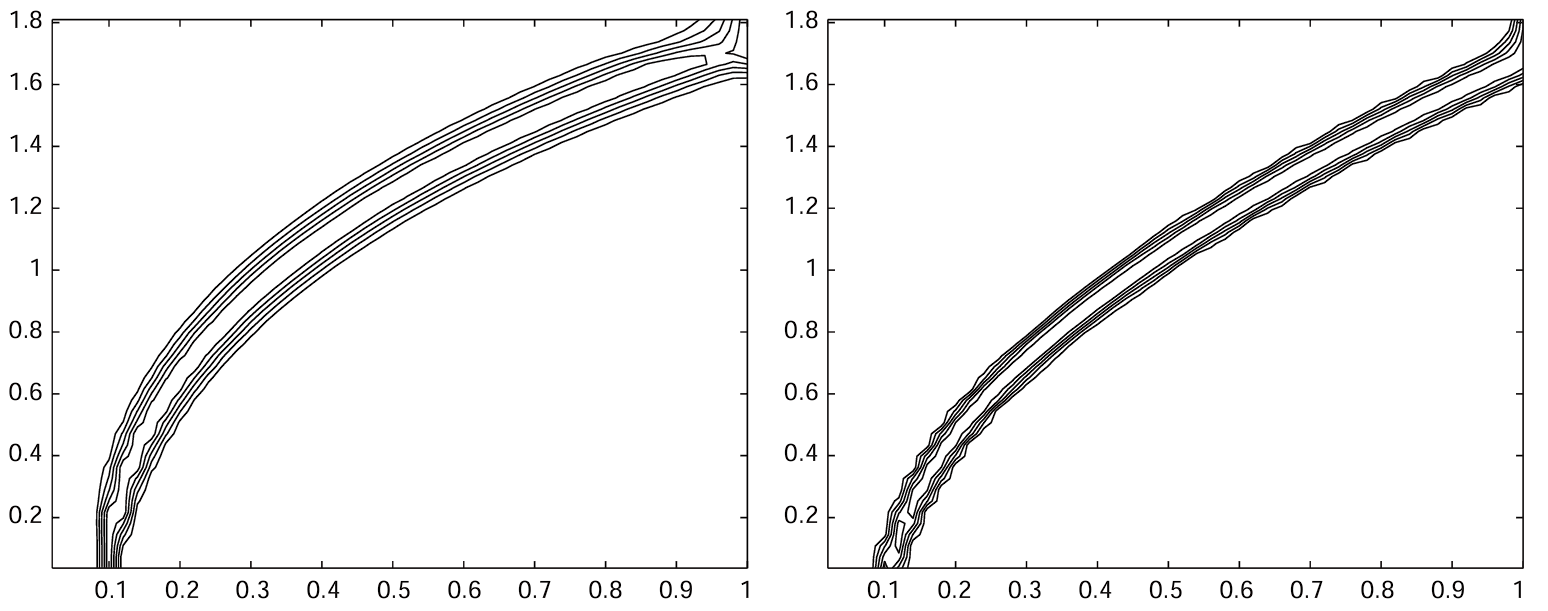
\includegraphics[scale=0.4]{image.png}
	\caption{Primera simulación. El eje $x$ es la característica y el eje $y$ es el tiempo. La población se especializa al consumo del primer nutriente ($\eta(x)=1/1-x$)\citep{dieckman2005}}
	\label{sim1}
\end{figure}

\begin{figure}[H]
	\centering
	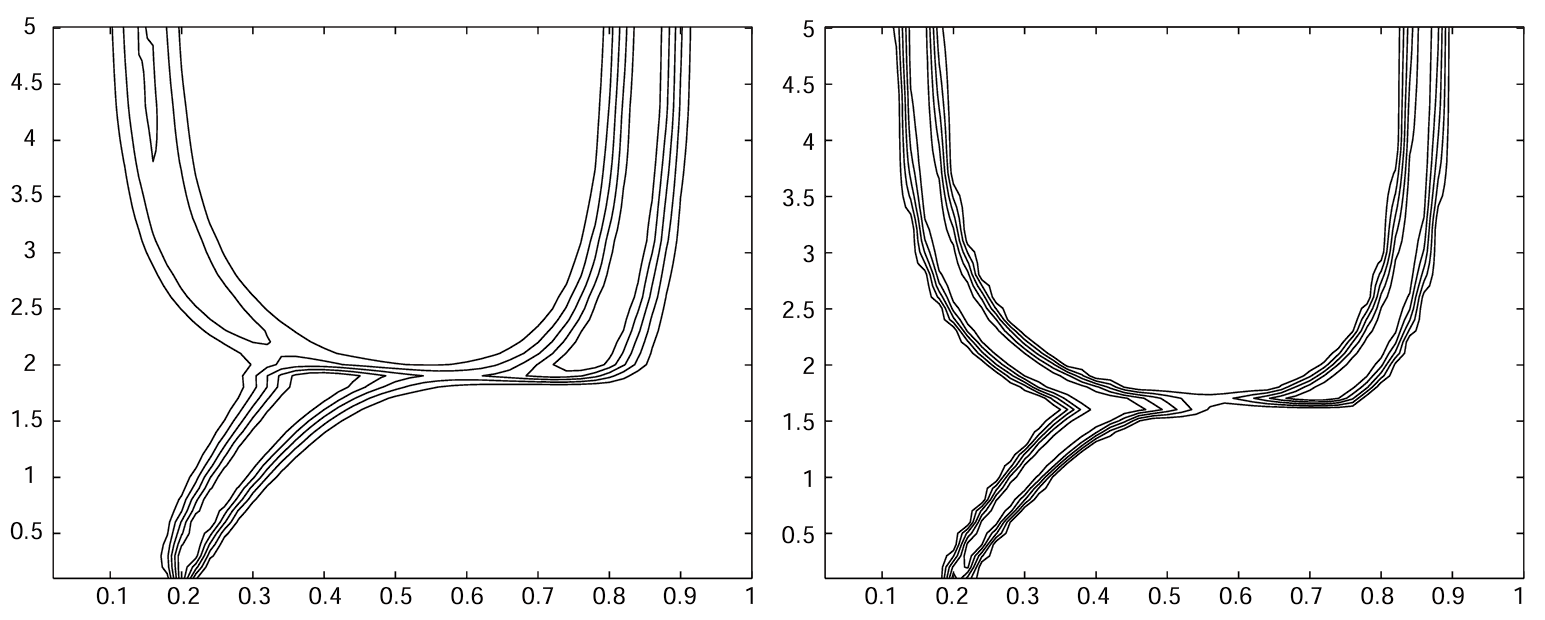
\includegraphics[scale=0.4]{Captura de pantalla 2024-12-11 095132.png}
	\caption{Segunda simulación. El eje $x$ es la característica y el eje $y$ es el tiempo. La especialización en el consumo se divide en dos dando una ramificación ($\eta(x)=x-1.8x(1-x)[x(1-x)-6/25]$, $\xi=1-x-1.8x(1-x)[x(1-x)-6/25]$)\citep{dieckman2005}}
	\label{sim2}
\end{figure}
Las gráfica Figura~\ref{sim1} y Figura~\ref{sim2} representan las líneas de nivel de la densidad de población en el espacio característica-tiempo.
\subsection{Resultados}
A partir del experimento numérico, se pueden ver varios resultados importantes que ayudan a comprender la dinámica de la población y su adaptación al ambiente.

Para el primer experimento encontramos:

\begin{enumerate}
	\item Tendencia hacia $x=1$: La densidad de la población muestra una inclinación hacia $x=1$, esto nos dice que, a medida que transcurre el tiempo, la población adapta su consumo para depender del nutriente 1, que es el único disponible. Este fenómeno refleja cómo las condiciones del ambiente obligan a la población a maximizar su supervivencia a través de un consumo más eficiente del recurso. Este comportamiento puede interpretarse como el efecto de un "potencial" ambiental que dirige la evolución adaptativa de la población hacia un estado óptimo.
	\item Estabilidad en tiempos largos: Conforme el tiempo avanza, la población parece alcanzar un estado de equilibrio en su densidad. La mayor parte de la población depende del nutriente 1.
	\item Forma logarítmica en el movimiento de la densidad: la trayectoria del movimiento de la densidad parece tener un comportamiento logarítmico, que empieza un crecimiento rápido de la adaptación y se va reduciendo a medida que la población se acerca al estado de equilibrio, la adaptación de una especie a su entorno, no presenta un comportamiento lineal en el tiempo.
\end{enumerate}

\textbf{Analogía con el movimiento de un frente de onda:} El movimiento de la densidad de la población en el espacio definido por la característica $x$ y el tiempo presenta una analogía interesante con la propagación de un frente de onda. Este frente parece desplazarse en la dirección positiva de $x$ a medida que el tiempo avanza, es similar a un frente de onda en un medio físico. Este enfoque permite interpretar el comportamiento de la densidad no solo como un proceso adaptativo, sino también como un fenómeno de propagación en este espacio.

Para el segundo experimento (con dos nutrientes) encontramos:
\begin{enumerate}
	\item Estabilidad y eficiencia en el consumo:
	      La densidad de la población muestra una tendencia a alcanzar la estabilidad y a maximizar la eficiencia en el consumo de los recursos disponibles. Esto refleja un comportamiento adaptativo general de la población frente a las condiciones del entorno.

	\item Aparición de un efecto de competencia:
	      La disponibilidad de dos nutrientes genera un fenómeno de competencia entre los miembros de la población. Como resultado, la población adapta su consumo dividiéndose en dos grupos: uno que se especializa en el consumo del nutriente 1 y otro que se especializa en el nutriente 2. Creemos que esta división es impulsada por la necesidad de optimizar el consumo y repartir los recursos de manera más eficiente, minimizando la competencia interna, esto hace posible formular este comportamiento en términos de un principio variacional.

	\item Especialización de las sub-densidades
	      Tras la división, las dos partes de la densidad de población (que, aunque forman parte de la misma población, pueden considerarse característicamente distintas) se especializan en el consumo de uno de los dos nutrientes. Este comportamiento permite una distribución más eficiente de los recursos en el sistema, reforzando la estabilidad del ambiente y la población.
\end{enumerate}

\textbf{Analogía como efecto de dispersión:}
A partir de la analogía con un frente de onda, observamos que el sistema genera un efecto que separa las densidades hacia $x=1$ y $x=0$, reflejando la especialización hacia cada uno de los nutrientes. Sin embargo, no podemos interpretar este comportamiento estrictamente como un fenómeno de onda, ya que no se observan características típicas de las ondas como la difracción, donde las superposiciones podrían generar efectos constructivos o destructivos. En lugar de ello, el sistema parece mostrar un efecto más cercano a un fenómeno de dispersión, en el que las densidades se separan sin interferencias mutuas significativas, y donde el parámetro de impacto parece estar dado por las características del consumo de los nutrientes, funciones $\eta(x),\:\xi(x)$.
\section{Conclusiones}

El formalismo de Hamilton-Jacobi puede extenderse a casos en los que la población inicial sea dimórfica, y se plantea que, de manera análoga, también podría aplicarse a poblaciones iniciales polimórficas.

Además, la solución numérica obtenida mediante el método directo se reproduce de manera equivalente a través de la solución a la ecuación de Hamilton-Jacobi asociada. Esto sugiere que este formalismo es aplicable a modelos con características similares.

Por lo anteriormente mencionado, es posible modelar fenómenos como la invasibilidad, sustituibilidad, entre otros, mediante este formalismo, incorporando constricciones, multiplicadores de Lagrange, y condiciones iniciales además de las ya establecidas.



\clearpage
\bibliographystyle{plainnat}
\bibliography{ref}
\end{document}
